\documentclass[tikz,border=6pt]{standalone}

% общий стиль (подключается через TEXINPUTS)
% tikz-style.tex (общий стиль для всех TikZ-картинок)
\RequirePackage[T1,T2A]{fontenc}
\RequirePackage[utf8]{inputenc}

% Palatino-подобный шрифт (как в MathJax часто воспринимается «более вытянутым»)
\RequirePackage{txfonts}
% txfonts даёт предупреждение по кириллице (T2A/txr не определён).
% Оставляем txfonts для математики, а текстовый шрифт возвращаем на Computer Modern,
% чтобы не искать T2A/txr и убрать предупреждения.
\renewcommand{\rmdefault}{cmr}
\renewcommand{\sfdefault}{cmss}
\renewcommand{\ttdefault}{cmtt}

\RequirePackage{tikz}
\RequirePackage{xcolor}
\usetikzlibrary{calc}

% цвета
\definecolor{lightgreen}{RGB}{214,234,214}
\definecolor{darkgreen}{HTML}{0B7A0B}
\definecolor{darkred}{HTML}{DF0000}

\definecolor{midgreen}{HTML}{2E9B2E}
\definecolor{palegreen}{RGB}{235,246,235}
\definecolor{olivegreen}{HTML}{3E6B2F}

\definecolor{lightred}{RGB}{255,220,220}
\definecolor{midred}{HTML}{E04545}
\definecolor{darkred2}{HTML}{A80000}

\definecolor{lightblue}{RGB}{220,232,255}
\definecolor{midblue}{HTML}{2E5BD6}
\definecolor{darkblue}{HTML}{0B2E8A}

\definecolor{lightgray}{RGB}{240,240,240}
\definecolor{midgray}{RGB}{170,170,170}
\definecolor{darkgray}{RGB}{80,80,80}

\definecolor{vtxfill}{RGB}{86,193,255}
\definecolor{vennfill}{RGB}{220,232,255}


% единый набор стилей TikZ
\tikzset{
    lab/.style={
        font=\fontsize{24}{32}\selectfont
    }
}


\begin{document}
  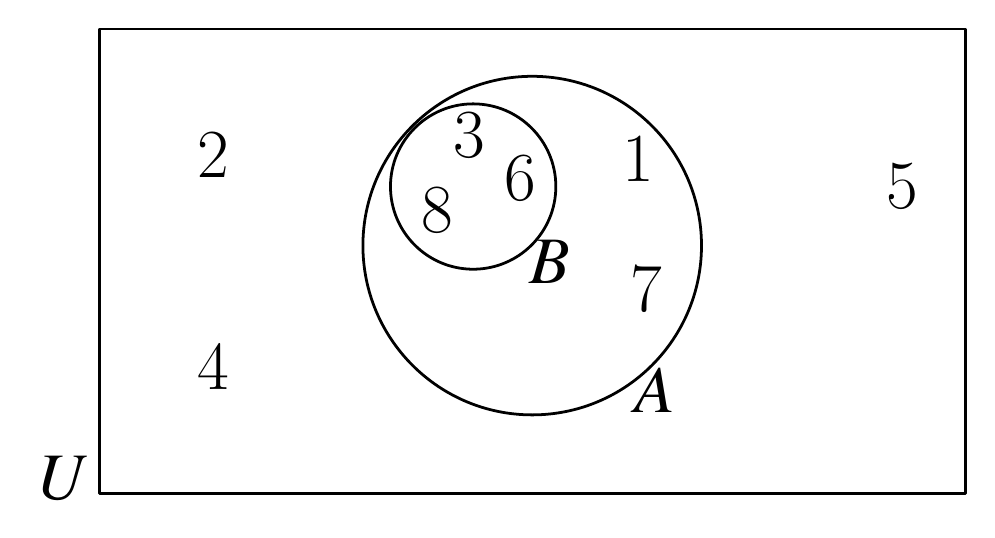
\begin{tikzpicture}[line cap=round,line join=round]

% --- geometry ---
    \def\RA{2.15}                       % radius of A (big circle)
    \def\RB{1.05}                       % radius of B (small circle)
    \coordinate (A) at ( 0.00,0.20);     % big circle center (centered)
    \coordinate (B) at (-0.75,0.95);     % small circle center (inside A)

% universe rectangle
    \draw[line width=1.0pt] (-5.5,-2.95) rectangle (5.5,2.95);

% circles (transparent interior)
    \draw[line width=1.0pt] (A) circle (\RA);
    \draw[line width=1.0pt] (B) circle (\RB);

% labels
    \node[lab] at ($ (A) + (1.55,-1.85) $) {$A$};
    \node[lab] at ($ (A) + (0.20,-0.20) $) {$B$};

% numbers outside A (but inside U)
    \node[lab] at (-4.05, 1.35) {2};
    \node[lab] at (-4.05,-1.35) {4};
    \node[lab] at ( 4.70, 0.95) {5};

% numbers inside A \ B
    \node[lab] at ($ (A) + (1.35, 1.10) $) {1};
    \node[lab] at ($ (A) + (1.45,-0.55) $) {7};

% numbers inside B
    \node[lab] at ($ (B) + (-0.05, 0.65) $) {3};
    \node[lab] at ($ (B) + ( 0.60, 0.10) $) {6};
    \node[lab] at ($ (B) + (-0.45,-0.30) $) {8};

% universe label (outside bottom-left of the rectangle)
    \node[lab, anchor=north east] at (-5.5,-2.35) {$U$};

  \end{tikzpicture}
\end{document}